%; whizzy chapter -dvi
% -initex iniptex -latex platex -format platex -bibtex jbibtex -fmt fmt
% 以上 whizzytex を使用する場合の設定。
 
%     Tokyo Debian Meeting resources
%     Copyright (C) 2012 Junichi Uekawa
%     Copyright (C) 2011 Nobuhiro Iwamatsu

%     This program is free software; you can redistribute it and/or modify
%     it under the terms of the GNU General Public License as published by
%     the Free Software Foundation; either version 2 of the License, or
%     (at your option) any later version.

%     This program is distributed in the hope that it will be useful,
%     but WITHOUT ANY WARRANTY; without even the implied warranty of
%     MERCHANTABILITY or FITNESS FOR A PARTICULAR PURPOSE.  See the
%     GNU General Public License for more details.

%     You should have received a copy of the GNU General Public License
%     along with this program; if not, write to the Free Software
%     Foundation, Inc., 51 Franklin St, Fifth Floor, Boston, MA  02110-1301 USA

%  preview (shell-command (concat "evince " (replace-regexp-in-string "tex$" "pdf"(buffer-file-name)) "&"))

%%ここからヘッダ開始。

\documentclass[mingoth,a4paper]{jsarticle}
\usepackage{monthlyreport}
% 日付を定義する、毎月変わります。
\newcommand{\debmtgyear}{2014}
\newcommand{\debmtgmonth}{12}
\newcommand{\debmtgdate}{20}
% started from zero:
% (let ((year 2013) (month 7)) (+ (* (- year 2005) 12) month -1))
\newcommand{\debmtgnumber}{121}

% tikz picture の為のマクロ設定
\usepackage[dvipdfmx]{graphicx}
\usepackage{tikz}

\begin{document}

\begin{titlepage}
\thispagestyle{empty}
% タイトルページ:編集必要な部分は最初のマクロに飛ばすこと

\vspace*{-2cm}
第\debmtgnumber{}回 東京エリア Debian 勉強会資料\\
\hspace*{-2cm}
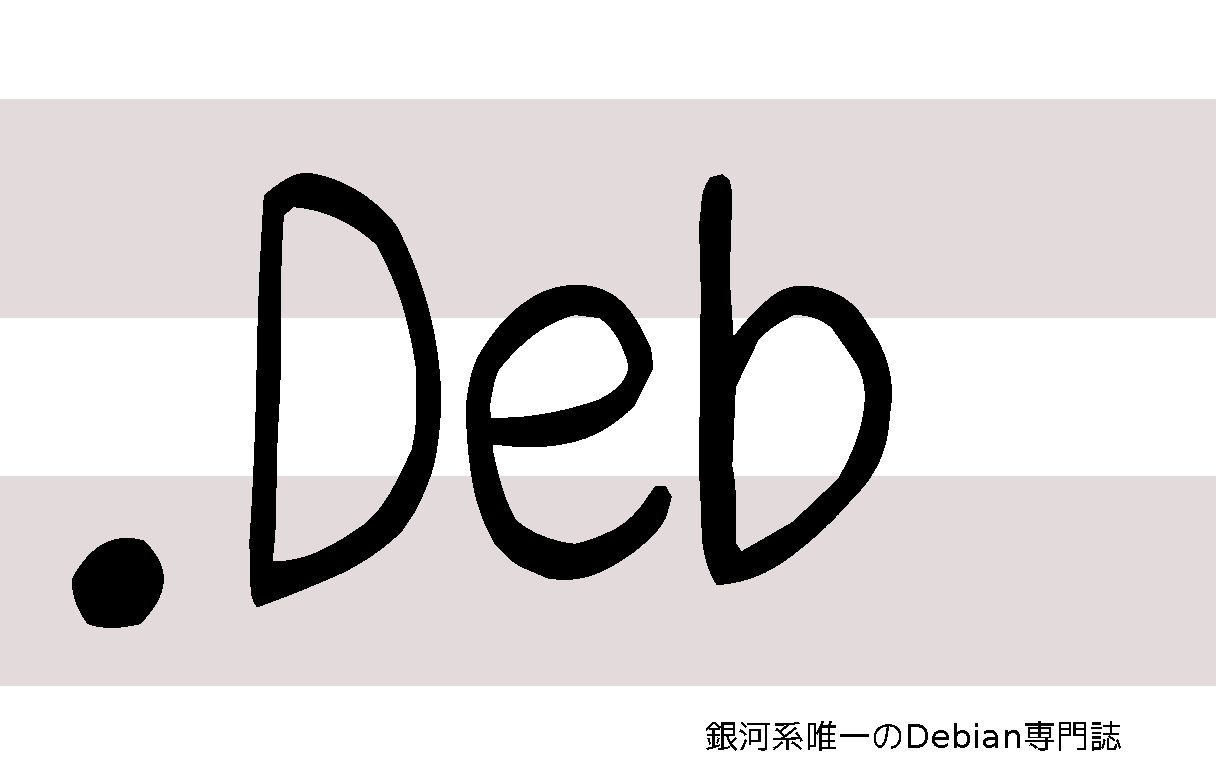
\includegraphics{image2012-natsu/dotdeb.pdf}\\
\hfill{}\debmtgyear{}年\debmtgmonth{}月\debmtgdate{}日

% ここはアップデートすること
% 全角文字にしないとフォントのサイズが合わないので注意
\rotatebox{10}{\fontsize{30}{30} {\gt 特集:DebianからみたLinux Mint}}\\

\vspace*{-2cm}
\hfill{}
\includegraphics[height=6cm]{image200502/openlogo-nd.eps}
\end{titlepage}

\newpage

\begin{minipage}[b]{0.2\hsize}
 \definecolor{titleback}{gray}{0.9}
 \colorbox{titleback}{\rotatebox{90}{\fontsize{80}{80} {\gt デビアン勉強会} }}
\end{minipage}
\begin{minipage}[b]{0.8\hsize}
\hrule
\vspace{2mm}
\hrule
\begin{multicols}{2}
\tableofcontents
\end{multicols}
\vspace{2mm}
\hrule
\end{minipage}

\dancersection{事前課題}{野島 貴英}

今回の事前課題は以下です:
\begin{enumerate}
\item どこで今回の勉強会の開催を知りましたか?
\item 何について聞きたい/参加者と話をしたいですか?
\item 本日、何の作業をやるかを宣言ください。
\end{enumerate}
この課題に対して提出いただいた内容は以下です。
\begin{multicols}{2}
{\small
\begin{prework}{ henrich }
  \begin{enumerate}
  \item Q.$B$I$3$G:#2s$NJY6/2q$N3+:E$rCN$j$^$7$?$+!)(B\\
    A. $BM'C#$dCN$j9g$$$+$iD>@\(B
  \item Q.$B2?$K$D$$$FJ9$-$?$$!?;22C<T$HOC$r$7$?$$$G$9$+!)(B\\
    A. \@kenhys$B$5$s$NOC$,3Z$7$_$G$9!*(B :)
  \item Q.hack time$B$K2?$r$7$^$9$+!)(B\\
    A. ($B2sEz$J$7(B)
  \end{enumerate}
\end{prework}

\begin{prework}{ $BLnEg(B }
  \begin{enumerate}
  \item Q.$B$I$3$G:#2s$NJY6/2q$N3+:E$rCN$j$^$7$?$+!)(B\\
    A. $B$=$NB>(B (Google$B8!:w%(%s%8%s$N8!:w7k2L$+$i(B)
  \item Q.$B2?$K$D$$$FJ9$-$?$$!?;22C<T$HOC$r$7$?$$$G$9$+!)(B\\
    A. $B$$$m$$$m$H!#;22C<T$H!#(B
  \item Q.hack time$B$K2?$r$7$^$9$+!)(B\\
    A. RC$BDY$7$H$+!"K]Lu$H$+!#(BRC$B$O(B\url{https://bugs.debian.org/release-critical/}$B;2>H!#(B
  \end{enumerate}
\end{prework}

\begin{prework}{ knok }
  \begin{enumerate}
  \item Q.$B$I$3$G:#2s$NJY6/2q$N3+:E$rCN$j$^$7$?$+!)(B\\
    A. Debian JP$B$N%a!<%j%s%0%j%9%H(B
  \item Q.$B2?$K$D$$$FJ9$-$?$$!?;22C<T$HOC$r$7$?$$$G$9$+!)(B\\
    A. key sign$B$d$j$^$9(B
  \item Q.hack time$B$K2?$r$7$^$9$+!)(B\\
    A. $B$$$/$D$+$N%=!<%9$N<L7P$H!"$G$-$l$P(BK\&R$B%9%?%$%k$NGS=|(B
  \end{enumerate}
\end{prework}

\begin{prework}{ koedoyoshida }
  \begin{enumerate}
  \item Q.$B$I$3$G:#2s$NJY6/2q$N3+:E$rCN$j$^$7$?$+!)(B\\
    A. Debian JP$B$N%a!<%j%s%0%j%9%H(B
  \item Q.$B2?$K$D$$$FJ9$-$?$$!?;22C<T$HOC$r$7$?$$$G$9$+!)(B\\
    A. $B%Q%C%1!<%8%s%0(B
  \item Q.hack time$B$K2?$r$7$^$9$+!)(B\\
    A. $B$^$C$?$j%a%s%F%J%s%9(B or $BK]Lu(B
  \end{enumerate}
\end{prework}

\begin{prework}{ kenhys }
  \begin{enumerate}
  \item Q.$B$I$3$G:#2s$NJY6/2q$N3+:E$rCN$j$^$7$?$+!)(B\\
    A. Twitter (@debianjp)
  \item Q.$B2?$K$D$$$FJ9$-$?$$!?;22C<T$HOC$r$7$?$$$G$9$+!)(B\\
    A. $B$f$/$f$/$O(BDebian$B$K0lK\2=$7$?$$$1$I2aEO4|$J$?$a(Bupstream$B$G(Bdebian,ubuntu$B8~$1$K%Q%C%1!<%8$rDs6!$7$F$$$k?M$N(Bdebian/$B4IM}=QE*$J%;%_%J!<$,J9$-$?$$(B
  \item Q.hack time$B$K2?$r$7$^$9$+!)(B\\
    A. porterbox$B$,$i$_$N2?$+(B
  \end{enumerate}
\end{prework}

\begin{prework}{ wbcchsyn }
  \begin{enumerate}
  \item Q.$B$I$3$G:#2s$NJY6/2q$N3+:E$rCN$j$^$7$?$+!)(B\\
    A. $BM'C#$dCN$j9g$$$+$iD>@\(B
  \item Q.$B2?$K$D$$$FJ9$-$?$$!?;22C<T$HOC$r$7$?$$$G$9$+!)(B\\
    A. $B:G6a$N>u67$K$D$$$F!">pJs8r49(B
  \item Q.hack time$B$K2?$r$7$^$9$+!)(B\\
    A. Debian $B$N3+H/4D6-9=C[(B
  \end{enumerate}
\end{prework}

\begin{prework}{ zinrai }
  \begin{enumerate}
  \item Q.$B$I$3$G:#2s$NJY6/2q$N3+:E$rCN$j$^$7$?$+!)(B\\
    A. $B$=$NB>(B
  \item Q.$B2?$K$D$$$FJ9$-$?$$!?;22C<T$HOC$r$7$?$$$G$9$+!)(B\\
    A. systemd
  \item Q.hack time$B$K2?$r$7$^$9$+!)(B\\
    A. drone+docker$B$G(BCI$B$r;n$7$F$_$k(B
  \end{enumerate}
\end{prework}

\begin{prework}{ alohaug }
  \begin{enumerate}
  \item Q.$B$I$3$G:#2s$NJY6/2q$N3+:E$rCN$j$^$7$?$+!)(B\\
    A. $B$=$NB>(B
  \item Q.$B2?$K$D$$$FJ9$-$?$$!?;22C<T$HOC$r$7$?$$$G$9$+!)(B\\
    A. Gnuk$B$N8=>u$N>R2p$,$7$?$$$G$9!#(B
  \item Q.hack time$B$K2?$r$7$^$9$+!)(B\\
    A. Gnuk$B$N%D!<%k:n$j$G%O%^$C$F$$$k$3$H$rAjCL$7$?$$$G$9!#(B
  \end{enumerate}
\end{prework}

\begin{prework}{ munepi }
  \begin{enumerate}
  \item Q.$B$I$3$G:#2s$NJY6/2q$N3+:E$rCN$j$^$7$?$+!)(B\\
    A. Debian JP$B$N%a!<%j%s%0%j%9%H(B
  \item Q.$B2?$K$D$$$FJ9$-$?$$!?;22C<T$HOC$r$7$?$$$G$9$+!)(B\\
    A. Debian$B$H(BFedora$B%Q%C%1!<%8%s%0$N$*OC(B
  \item Q.hack time$B$K2?$r$7$^$9$+!)(B\\
    A. $BJY6/2q;qNAMQ(B\LaTeX $B%9%?%$%k$N2~A1!"%/%i%9%U%!%$%k$N:n@.!J0F!K(B
  \end{enumerate}
\end{prework}

\begin{prework}{yy\_y\_ja\_jp }
  \begin{enumerate}
  \item Q.$B$I$3$G:#2s$NJY6/2q$N3+:E$rCN$j$^$7$?$+!)(B\\
    A. $B$=$NB>(B
  \item Q.$B2?$K$D$$$FJ9$-$?$$!?;22C<T$HOC$r$7$?$$$G$9$+!)(B\\
    A. Debian
  \item Q.hack time$B$K2?$r$7$^$9$+!)(B\\
    A. DDTSS(\url{http://ddtp.debian.net/ddtss/index.cgi/ja})
  \end{enumerate}
\end{prework}

}
\end{multicols}

\dancersection{Debian Trivia Quiz}{野島 貴英}

 Debianの昨今の話題についてのQuizです。

今回の出題範囲は\url{debian-devel-announce@lists.debian.org} や \url{debian-news@lists.debian.org}に投稿された
内容などからです。

\begin{multicols}{2}
%; whizzy-master ../debianmeetingresume201311.tex
% $B0J>e$N@_Dj$r$7$F$$$k$?$a!"$3$N%U%!%$%k$G(B M-x whizzytex $B$9$k$H!"(Bwhizzytex$B$,MxMQ$G$-$^$9!#(B
%

\santaku
{2014/11$B7nCf=\$K$F(BDebconf15$B$N%9%]%s%5!<$H$J$C$?4k6H$O2?<R$"$k$G$7$g$&!)(B}
{3$B<R(B}
{9$B<R(B}
{11$B<R(B}
{C}
{$B%9%]%s%5!<4k6H0lMw!'(Bcredativ, sipgate, Matanel Foundation, Google,
Fairsight Security, Martin Alfke / Buero 2.0, Ubuntu, Mirantis, Logilab,
Netways,Hetzner$B!#$5$"!*F|K\4k6H$N3'MM$b@'Hs$40l=o$K!*(B}

\santaku
{2014/11/18$B$K?k$K%0%i%UI=<(5!G=IU$-EEBn$G(BDebian$B$rF0$+$7$?6/<T$,8=$l$?;v$,OCBj$K$J$C$F$$$^$7$?!#;H$o$l$?EEBn$N%a!<%+$O$I$l!)(B}
{Texus Instruments$B<R(B}
{CASIO$B<R(B}
{Hewllet Packard$B<R(B}
{A}
{$B>\$7$/$O!'(Bhttp://hackaday.com/2014/11/18/ running-debian-on-a-graphing-calculator/$B!#;H$o$l$?EEBn$N@=IJL>$O!'(BTI-NSpire CX$B$H$$$&%7%j!<%:$N5!<o$@$=$&$G$9!#(B}

\santaku
{Debian$B%W%m%8%'%/%H$K$F(Binit$B%7%9%F%`$N%"%W%j%1!<%7%g%s$N0MB8EY$K4X$9$k(BGeneral Resolution$B$NEjI<$,9T$o$l$^$7$?!#EjI<$N7k2L$O!)(B}
{$B%Q%C%1!<%8$OFCDj$N(Binit$B%7%9%F%`$N$_$K0MB8$7$F$O$J$i$J$$(B}
{$B%Q%C%1!<%8%a%s%F%J$,K>$a$P!"FCDj$N(Binit$B%7%9%F%`$K0MB8$7$F$b(BOK}
{General Resoultion$B$OITMW$@(B}
{C}
{Debian$B$G$b(Binit system$B$H%Q%C%1!<%8$H$ND4@0$,0z$-B3$-0l@87|L?9T$o$l$F$$$^$9!#(B}

\santaku
{Debian Med$B%a%?%Q%C%1!<%8$N%P!<%8%g%s$,(B1.99$B$X0l5$$K%8%c%s%W$9$kM=Dj$G$"$k$3$H$,%"%J%&%s%9$5$l$^$7$?!#$3$N;~=i$a$FEk:\$5$l$kM=Dj$N0eNE4X78<T8~$1%7%9%F%`$O2?!)(B}
{$B0dEA;R2r@O%7%9%F%`(B}
{$B302J<j=QMQ%m%\%C%H%7%9%F%`(B}
{$BIB1!>pJs%7%9%F%`(B(HIS)}
{C}
{Debian Med$B%A!<%`$N:#2s$N4hD%$j$OAG@2$i$7$/!"(BPHYLP$B$N%i%$%;%s%9$rD9G/$N8r>D$NKv!"(BDFSG$B=`5r$N$b$N$KJQ99$7$F$b$i$&$J$I!"0eNE4X78<T$i!&@8J*3X4X78<T$i$KMM!9$K%]%8%F%#%V$J1F6A$rM?$($F$$$^$9!#$3$N3hF0$O0eNEJ,Ln$N3X=Q7O$N>pJs%5%$%H(BBioMedCentral$B$K(B''Community-driven development for computational biology at Sprints, Hackathons and Codefests''$B$H$$$&$3$H$G<h$j>e$2$i$l$?$=$&$G$9!#(B}

\santaku
{2014/11/14$B$K(BDebian$B$N(BBTS$B$K!"(BDebian$B$N%Q%C%1!<%83+H/=i?4<T$X=$@5:n6H$,NI$$1i=,$H$J$k$h$&$J%P%0$K4X$9$k(Btag$B$,@_$1$i$l$^$7$?!#0J2<$N$I$l(B}
{newcomer}
{gift}
{easeofcake}
{A}
{$B:#$^$G%Q%C%1!<%83+H/=i?4<T8~$1$K3d$jEv$F$i$l$F$$$?(BBTS$B$N(Btag$B$O(Bgift$B$G$7$?$,!"(Bnewcomer$B$XJQ$o$k$=$&$G$9!#0JA0$N(Bgift$B$H$$$&(Btag$BL>$@$H$A$g$C$HH=$j$K$/$$$H$N$3$H$G!":#2sL>A0JQ99$H$J$C$?$h$&$G$9!#(B}

\santaku
{Mysql$B$K4X$9$k2>A[%Q%C%1!<%8$KDj5A$5$l$?(BMysqlDB$B8_49(BDB$B%=%U%H$H$7$F(BPXC$B$H$$$&$N$,$"$k$,!"$3$A$i$O2?$NN,!)(B}
{Protected eXchange Controler}
{Posgresql eXtra Controler}
{Percona XtraDB Cluster}
{C}
{Debian$B$K$F!"(BMysql$B7O$N(BDB$B$H$_$J$5$l$?$b$N$O!"#3$D$"$j!"(BMysqlDB,MariaDB,Percona XtraDB Cluster(PCX)$B$N#3$D$H$J$j$^$9!#(B}

\santaku
{2014/11/20$B$K$F!"(Bsystemd$BMQ$NDj5A%U%!%$%kFbIt$G;H$($k%;%-%e%j%F%#$rBgI}$K8~>e=PMh$k%*%W%7%g%s$N$&$A!"%[!<%`%G%#%l%/%H%j$NIT@5%"%/%;%9$rM^;_$9$k$N$O<!$N$I$l(B}
{ProtectHome}
{ProtectSystem}
{PrivateTmp}
{A}
{systemd$B$NDj5A%U%!%$%k$KMQ0U$5$l$F$$$k%;%-%e%j%F%#$K4X$9$k%*%W%7%g%s$r$&$^$/;H$$$3$J$9$HHs>o$K6/8G$J%7%9%F%`$K$9$k$3$H$,=PMh$k$=$&$G$9!#%N%&%O%&$H>R2p$O(Bhttp://0pointer.net/public/systemd-nluug-2014.pdf}















\end{multicols}

\dancersection{最近のDebian関連のミーティング報告}{野島 貴英}

\subsection{第120回東京エリアDebian勉強会}

\begin{itemize}
\item 場所はスクウェア・エニックスさんのセミナルームをお借りしての開催でした。
\item 参加者は10名でした。
\item セミナ内容は野島により、DebianとArch Linuxの比較を行ったことについて語りました。
\item 残りの時間でhack timeを行い、成果発表をしました。
\item 宴会の代わりに、「やよい軒 新宿明治通り店」で夕食会をやりました。
\end{itemize} 

 前回のセミナですが、OSC Tokyoにてブースを出していると若いLinuxユーザの方がArch Linuxを使っている割合が高いことから、調べてみました。何故人気があるのか、Debianとどう違い、どういうニーズがあるのか?について考察できたように思います。他のディストリビューションと比較すると、Debianの立ち位置、取り込んだ方が良い機能などがわかって良いかと思います。

% % (query-replace-regexp "<.*?>" "")
% % (query-replace-regexp "^[	 ]\+" "")

%-------------------------------------------------------------------------------
\dancersection{DebianからみたLinux Mint}{野島 貴英}
%-------------------------------------------------------------------------------
\index{debian-arch-linux}

\subsection{はじめに}

 OSC\footnote{\url{http://www.ospn.jp/}}にて、ブースを出した際、様々な来場者の方々と意見交換をしています。この時印象深かった事として、特に若い年齢の方々が、以下のディストリビューションを使っているようです。

 \begin{itemize}
 \item Arch Linux
 \item Linux Mint
 \end{itemize}
 
 Debianはコミュニティー主導により進化し続けるディストリビューションです。他のディストリビューションにある良い点、Debianにある他のディストリビューションとの比較で悪い点、Debianの目指すべき立ち位置などは、他のディストリビューションとの比較でわかることも多いです。これらの違いを比較して、取り込むべき良い点があるのであれば、Debianに取り込まれるべきと考えます。

 今回、OSCの件もあり、ちょうど良い機会なので、先月のArch Linuxに続き、今月はLinux Mintを題材に、Debianとどのような違いがあるのかを調べてみました。

\subsection{Linux Mintとは}

 Linux Mintは、2006年に誕生しました\cite{ref:linuxmint-history}。UbuntuあるいはDebianをベースにして作られています。

 軽量で、かつ、Ubuntu/Debianをベースとしながら、Ubuntu/Debianではポリシー上提供しないようなプロプライエタリなドライバ/マルチメディア系ライブラリも予め搭載されています。初心者にも使いやすい事を狙いとして作られているディストリビューションです。

\subsection{Debian上の仮想環境にインストールしてみる}

ここではKVMを使ってDebian上にLinux Mintをインストールしてみます。なお、Linux MintのISOイメージは、基本的にLiveイメージでもあり、インストーラはこのLiveイメージに梱包されている通常のアプリケーションとなります。

Linux Mintはいくつかの種類にわかれたインストール用のISOイメージが用意されています。

\begin{itemize}
\item 導入されるデスクトップ環境別にイメージがあり、cinnamon版、MATE版、xfce版、KDE版があります。
\item 梱包されているマルチメディア用ミドルウェアについて、国によっては配布が違法となってしまうもの(例:libdvdcss等)を含んでいるため、これらを全て排除したNOCODEC版がそれぞれ用意されています。日本で使うのであれば、法的問題からNOCODEC版をおすすめします\cite{ref:linuxmint-illeagal-prog}。
\item 基本はUbuntuをベースにしていますが、Debianをベースにした物(LMDE)もあります。
\end{itemize}

ここでは、最近リリースされたLinux Mint 17.1(Rebecca)のMATE Nocodecの64bit版をdebian sid上に導入したKVMで動作させてみます。なお、Cinnamon版ですが、筆者の元ではvirt-viewerとの相性が非常に悪かった(cirrusエミュレーション及び、qxlエミュレーション共に)為、評価は断念しました。

\begin{description}
\item [Step 1.] DebianマシンにKVM/libvirt/virtinstをインストールしておきます。
  \begin{commandline}
$ sudo aptitude install qemu-kvm libvirt-bin virtinst
   \end{commandline}
\item [Step 2.] 今回使うISOイメージファイルである、linuxmint-17.1-mate-nocodecs-64bit.isoをダウンロードしておきます。
\item [Step 3.] 仮想ディスクを9GBytes以上の大きさで作成し、virt-installコマンドで起動します。また、guest OSへ割り当てる仮想メモリは1GBytes以上は用意しておかないとインストーラが途中で終了(OOM killerで強制終了)したりします。なお、ネットワークデバイスとして指定しているbr0はbridge/NATが有効でかつ、dnsmasqでDHCP/DNSが有効にしてあります。(参考文献:\cite{ref:kde-devel-debian}、\cite{ref:dnsmasq})
     \begin{commandline}
$ sudo qemu-img create -f raw /var/lib/libvirt/images/mint-01 9G
$ sudo virt-install --connect=qemu:///system -n mint-01 --ram 1024 \
     --cdrom /home/yours/arch-linux/linuxmint-17.1-mate-nocodecs-64bit.iso \
     --disk /var/lib/libvirt/images/mint-01,bus=virtio,size=9,format=raw,cache=writeback \
     --vnc --hvm --accelerate --bridge=br0,model=virtio
   \end{commandline}
   \item [Step 4.] Linux MintがMATEデスクトップ環境にてユーザmint権限の元ログイン済み立ち上がります(図\ref{fig:mint-boot})。
   \item [Step 5.] デスクトップ上にある、インストーラのアイコンをクリックしてインストーラを立ち上げ、表示される質問に答えていきます。質問全部に答えるとインストールが開始されます(図\ref{fig:mint-inst})。
   \item [Step 6.] インストールが完了するとリブートを促されますので、リブートします。
   \item [Step 7.] ログインし、「設定」→「Languages」にて、日本語IMの導入メニューがあるので、好きなIMを選んで追加のパッケージを導入して下さい。導入完了後、「Input method」プルダウンを導入したIMが選択されているようにしておきます(図\ref{fig:mint-im-setup})。
   \item [Step 8.] 再度リブートします。
   \item [Step 9.] 再度ログインすると、導入した日本語のIMが使えるようになっています(図\ref{fig:mint-setupcomplete})。
\end{description}
\begin{figure}[H]
\begin{minipage}{0.5\hsize}
\centering
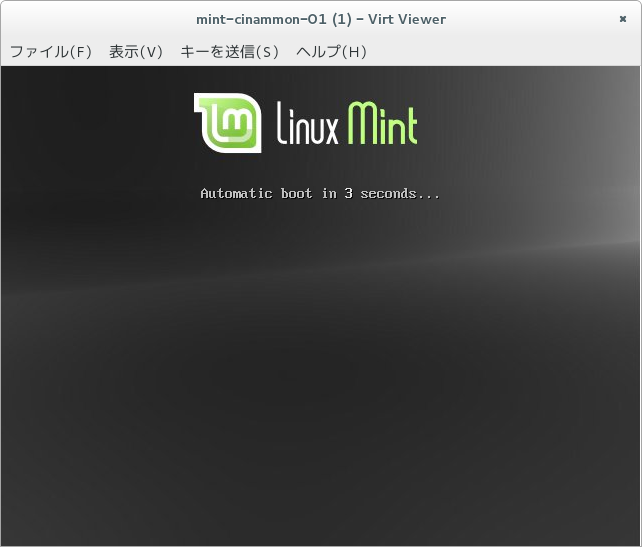
\includegraphics[width=0.8\hsize]{image201412/mint-inst-boot.png}
\caption{ブートの様子}\label{fig:mint-boot}
\end{minipage}
\begin{minipage}{0.5\hsize}
\centering
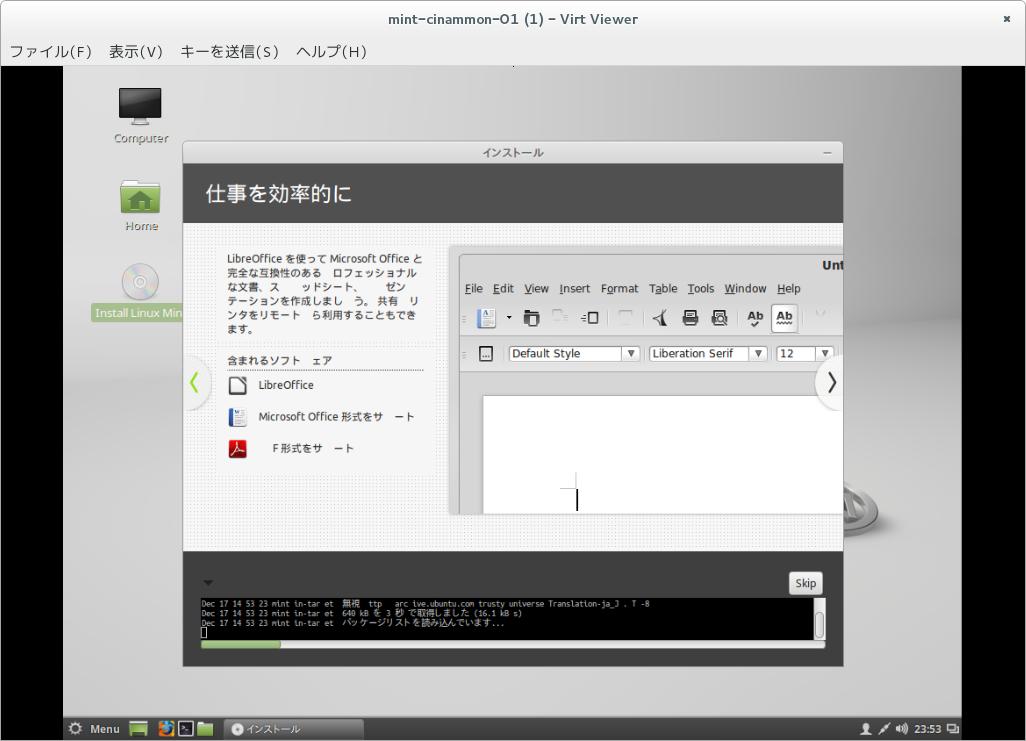
\includegraphics[width=0.8\hsize]{image201412/mint-inst.png}
\caption{インストーラ起動の様子}\label{fig:mint-inst}
\end{minipage}
\end{figure}
\begin{figure}[H]
\begin{minipage}{0.5\hsize}
\centering
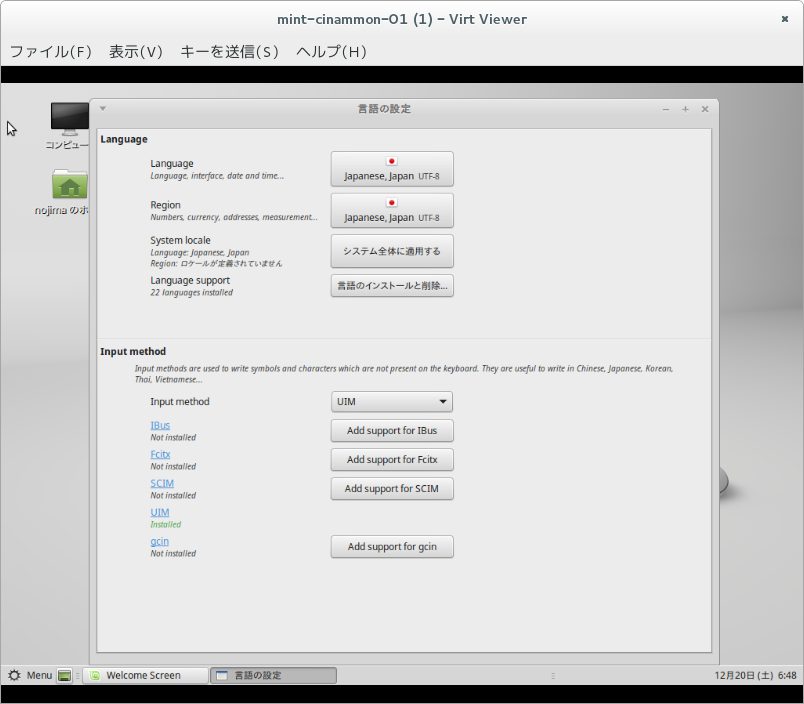
\includegraphics[width=0.8\hsize]{image201412/mint-im-setup.png}
\caption{日本語IM導入の様子}\label{fig:mint-im-setup}
\end{minipage}
\begin{minipage}{0.5\hsize}
\centering
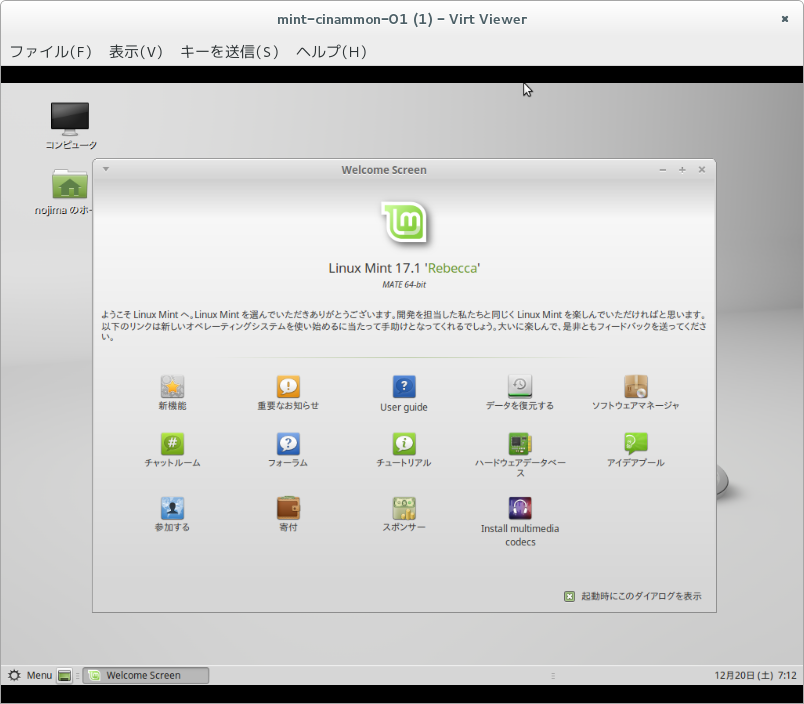
\includegraphics[width=0.8\hsize]{image201412/mint-setupcomplete.png}
\caption{インストール完了}\label{fig:mint-setupcomplete}
\end{minipage}
\end{figure}

 \subsection{Linux MintとUbuntu/Debianの関係}

 図\ref{fig:mint-construct}にLinux MintとUbuntu/Debianの関係を図示しておきます。Linux Mint側ではデスクトップ環境及びMintToolsのみをLinux Mint側で開発しており、残りの足らない部分をすべてUbuntuのパッケージから導入しているという作りとなります。

 このため、パッケージの更新を行う場合、Debianで行うように、うっかりapt-get/aptitudeなどでfull-upgradeすると、Linux Mintでは意図していない形で副作用のあるパッケージがうっかり導入されてしまう事があるため、パッケージの更新の時は「システム管理メニュー」の「アップデートマネージャ」を使ってアップグレードしなければならない等の制約があります。
\begin{figure}[H]
\centering
\includegraphics[width=0.8\hsize]{image201412/mint-construct.eps}  
\caption{Linux MintとUbuntu/Debianの関係}\label{fig:mint-construct}
\end{figure} 

\subsection{Linux Mintの良い所} 

以下にLinux Mintの良い所を載せます。

\begin{itemize}
 \item Linux Mint側でメンテナンスされている部分の作りが非常に丁寧であり、通常の利用であれば、GUIのメニューを操作するだけですぐに使えるのが良い点です。他ディストリビューション(Debian含む)のようにメニューの各項目の動作が不完全、あるいはメニューの項目が不完全ということは非常に少ないように思えます。
 \item Linux Mint側のcommunityサイト\footnote{\url{http://community.linuxmint.com/}}には、投票システムや、ユーザの投稿のランキングなどの様々な統計がすぐにみれるようになっています。さらに、アイデアの投稿場所があり、こちらに投稿されたアイデアについて、他のユーザが好感度を投票でき、どのアイデアが他のユーザに評価が高いかがすぐにわかるようになっています。
\end{itemize}

\subsection{cinnamonをDebian unstableに導入してみる}

 2014/9/4にDebianのtestingにLinux Mintで利用されている
デスクトップ環境であるcinnamonが入ったとのアナウンスがありました。

 ひょっとして、Debianにcinnamonを入れると、Linux Mintそっくりになったりするのかも?と思い、試しにDebian sidへ導入してみました。

\begin{description}
\item [Step 1.] Debian sidをデスクトップ環境を全く導入しない最小限の構成で導入します。
\item [Step 2.] cinnamonデスクトップ環境を導入します。
  \begin{commandline}
$ sudo aptitude install cinnamon-desktop-envirionment
  \end{commandline}
\item [Step 3.] Debina sidをリブートします。すると、lightdmが立ち上がり、ログイン画面が現れます。
\item [Step 4.] ログインすると、Debianらしいルックアンドフィールでcinnamonのディスクトップ環境が動作します。(図\ref{fig:debian-cinnamon})
\end{description}

 使うとわかるのですが、Debianの他デスクトップ環境の完成度としては普通の完成度です。Debianに慣れているのであれば、Debianで導入出来る他デスクトップ同様、管理の流儀も利用も全く違和感がありません。しかしながら、Linux Mintで提供されている程の、システム全体との統合はメニュー構成も含めて実現出来ていない状況です。このため、仮にLinux MintユーザがDebianへ乗り換えることを考えた場合、Debianにcinnamonを導入してみても、物足りなさを感じてしまうかも?と思いました。

\begin{figure}[H]
\centering
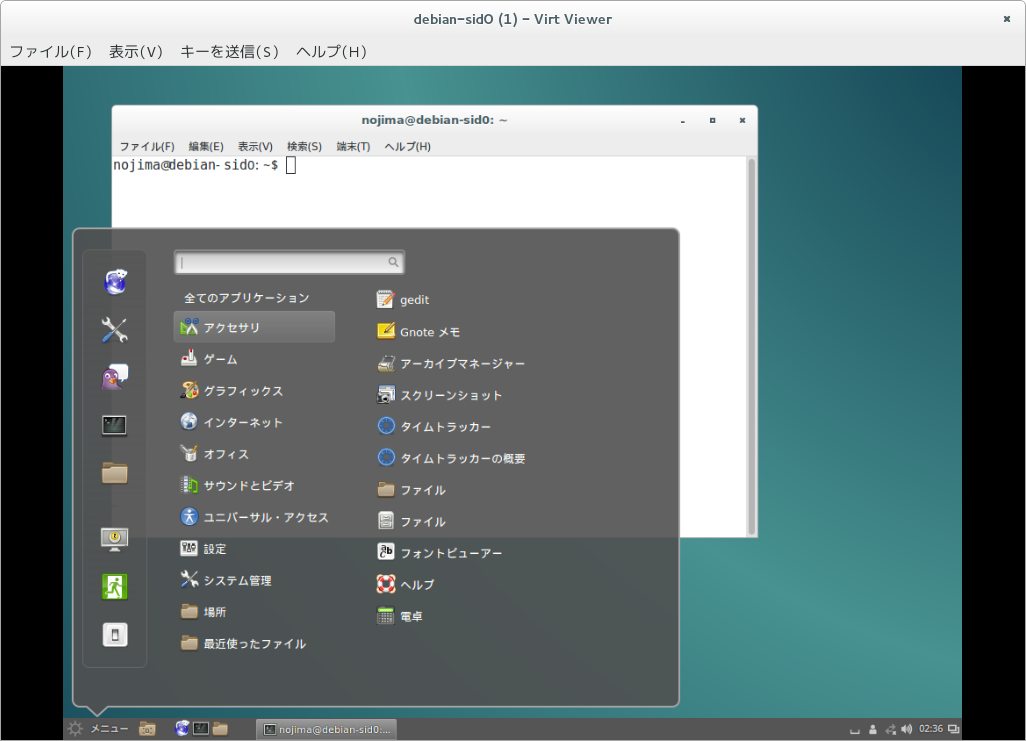
\includegraphics[width=0.6\hsize]{image201412/debian-cinnamon.png}  
\caption{Debianにcinnamonを導入した様子}\label{fig:debian-cinnamon}
\end{figure} 

\subsection{おわりに}

 今回は、Linux MintについてDebianからの視点で見てみました。Linux Mint communityのサイト、Linux Mint並にGUIとシステム管理が丁寧に統合されたデスクトップ環境の構成はDebianを考える上で非常に参考になります。将来こういった点をDebianで導入・改善していくと良いと思いました。

\begin{thebibliography}{9}
\bibitem{ref:linuxmint-history} Linux Mint UserGuide中 Historyの章,\url{http://www.linuxmint.com/documentation/user-guide/MATE/english_4.0.pdf}
\bibitem{ref:linuxmint-illeagal-prog} 「Linux Mintのミラーを再開しました」,\url{http://ftp-admin.blogspot.jp/2013/06/linux-mint.html}
\bibitem{ref:kde-devel-debian}「Debian開発者のKDE環境あれこれ」 第85回東京エリアDebian勉強会資料,\url{http://tokyodebian.alioth.debian.org/pdf/debianmeetingresume201202.pdf}
  \bibitem{ref:dnsmasq}「Debianでdnsmasqを使う」 第109回東京エリアDebian勉強会資料,\url{http://tokyodebian.alioth.debian.org/pdf/debianmeetingresume201402.pdf}
\end{thebibliography}
 
\newpage

\vspace*{15cm}
\hrule
\vspace{2mm}

\includegraphics[width=2cm]{image200502/openlogo-nd.eps}
\noindent \Large \bf Debian 勉強会資料\\
\noindent \normalfont \debmtgyear{}年\debmtgmonth{}月\debmtgdate{}日 \hspace{5mm}  初版第1刷発行\\
\noindent \normalfont 東京エリア Debian 勉強会 (編集・印刷・発行)\\
\hrule

\end{document}
